\documentclass[runningheads]{llncs}

\usepackage[T1]{fontenc}
\usepackage[utf8]{inputenc}
\usepackage{amsmath}
\usepackage{graphicx}
\usepackage{lettrine}
\usepackage{hyperref}
\usepackage{longtable}
\usepackage{subcaption}
\usepackage{float}

\begin{document}

\title{Single-Cell Transcriptomic Analysis of Zebrafish Pigment Cells}
\titlerunning{Single-Cell Transcriptomic Analysis of Zebrafish Pigment Cells}

\author{Diogo Esteves\inst{1}\orcidID{0000-0001-5741-5686} \and David Henriques\inst{2}\orcidID{0000-0002-9477-292X}}
\authorrunning{Esteves, D. \& Henriques, D.}

\institute{
    Department of Informatics, University of Minho, Portugal \\
    \email{pg28935@uminho.pt} \and
    CSIC IIM, Vigo, Spain \\
    \email{davidh@iim.csic.es}
}

\maketitle

\begin{abstract}
Zebrafish (\textit{Danio rerio}) is a model organism for understanding disease processes and vertebrate development. Their distinct coloring patterns provide valuable insights into genetic regulation and cellular differentiation. This study employs single-cell transcriptomics to analyze the complexity of pigment cell formation in zebrafish, providing new insight into cellular heterogeneity and gene expression. I hope to elucidate the mechanisms involved in pigment cell development by using cutting-edge methods like scRNA-seq and sophisticated analytical approaches such as UMAP and PCA, with a focus on the role of transcription factors and genetic networks. This complete approach is essential for the study of genetic variation and cellular development in this well-studied model species.
\end{abstract}

\section{Introduction}
\lettrine{P}{\newline}igmentation of \textit{Danio rerio} cells could offer valuable insights into genetic and developmental processes. \textit{D. rerio} is a key model organism in biology. Understanding its genetic regulation and cellular differentiation may be visually determined by its distinct pigmentation patterns, which are regulated by several types of pigment cells. Single-cell transcriptomics provides a comprehensive view of cellular heterogeneity and gene expression patterns, beyond standard bulk mRNA sequencing methodologies that fail to capture the cellular complexity and dynamic nature of live tissues \cite{kulkarni2019beyond}.

The zebrafish is commonly employed in genetic and developmental biology due to a variety of advantages, including transparent embryos, rapid development, and the capacity to generate a high number of offspring. These features make in vivo imaging and high-throughput genetic screening easier. Zebrafish are an ideal model for researching vertebrate development and disease mechanisms because of their genetic similarity to humans \cite{howard2021atlas,patterson2019zebrafish}.

In zebrafish, neural crest (NCs) cells generate pigment cells: melanophores (black), xanthophores (yellow), and iridophores (iridescent). 
These pigment cells are not only necessary for the striping pattern of zebrafish, but also serve as a model to understand processes of cell differentiation, migration, and survival \cite{patterson2019zebrafish}. 
The precise arrangement and interaction of these cells is essential for the development of the pigment pattern, making zebrafish an ideal vehicle for researching pigment cell biology. Single-cell RNA sequencing (scRNA-seq) has transformed the study of transcriptomics by allowing gene expression analysis and research at the level of individual cells. This approach provides insights into cellular heterogeneity and gene expression dynamics, allowing for the identification of diverse cell types and states within a tissue. ScRNA-seq has greatly improved our understanding of developmental processes and disease mechanisms at the cellular level \cite{nayak2021hitchhiker}.

The 10x Genomics Chromium system, have increased the accuracy, precision, and "output" of single-cell studies.
These technologies enable the profiling of thousands to millions of cells in a single experiment, resulting in a thorough understanding of cellular diversity and function. Integrating scRNA-seq data with other omics data, such as epigenomics and proteomics, enables a more comprehensive understanding of cellular regulation and interaction networks \cite{stuart2019comprehensive}.

Pigmentation in vertebrates is controlled by a complex balance of genetic and environmental variables. Pigmentation in zebrafish is regulated by multiple genes and signaling pathways, including transcription factors like MITF (Microphthalmia-associated transcription factor) and receptors like KIT (stem cell factor receptor). Pigment cells rely on these for development, survival, and function. Understanding the genetic basis of pigmentation provides knowledge in several biological processes, including cell differentiation, development, and illness \cite{kenny2022tfap2}.

\subsection*{Objective}
The primary objective of this study is to analyze the transcriptome of zebrafish pigment cells using single-cell RNA sequencing (scRNA-seq). The goal was to elucidate the genetic and molecular factors involved in pigment cell development by employing advanced analytical approaches such as UMAP (Uniform Manifold Approximation and Projection) and PCA (Principal Component Analysis). The study aimed to understand the role of transcription factors and genetic networks in regulating pigment cell differentiation and function. For the proposed schedule before some challenges appeared due to time and equipment limitations. It lewd to multiple changes and attempts in our objective approach, in powerful time-consuming script runs, more explanations in further sections.

\section{Background} 
The zebrafish (\textit{Danio rerio}) is an important model organism in biomedical research because of its genetic closeness to humans and practical advantages, including rapid development, transparency throughout embryonic stages, and high fertility. These traits help investigate developmental processes, genetic roles, and disease models \cite{howard2021atlas}.

Zebrafish embryos' transparency enables real-time monitoring of developmental processes, making them ideal for studying cellular dynamics and interactions. Furthermore, zebrafish's rapid development cycle, in which major organ systems arise within days, allows for quick turnaround for experimental experiments, making it a very efficient model organism \cite{patterson2019zebrafish,lencer2021single}.

Zebrafish pigment cells, originating from the NCs, are an excellent model for investigating cell differentiation and pattern generation. The NCs is a transient, multipotent, migrating cell population unique to vertebrates, originating a large variety of cell types, including neurons, glia, and pigment cells \cite{subkhankulova2023zebrafish}. 

These NCs cells travel throughout the organism and develop into many cell types, including pigment cells, which are required for the zebrafish's distinctive striping pattern. This migration and differentiation process is tightly controlled and involves a complex interaction of genetic and environmental factors\cite{patterson2019zebrafish}.

Pigmentation is regulated by a complex network of genes. Key transcription factors, such as MITF (Microphthalmia-associated transcription factor), help melanophores develop and operate by controlling genes involved in melanin synthesis and pigment cell survival. KIT, a receptor tyrosine kinase, promotes pigment cell migration and survival \cite{kenny2022tfap2,jang2021epigenetic}. 

Mutations or alterations in these pathways can induce pigmentation abnormalities and lead to a variety of pigmentation illnesses, highlighting the importance of these components in normal pigment cell growth and function. For example, mutations in the MITF gene can cause Waardenburg syndrome, which is characterized by pigmentary abnormalities and hearing loss \cite{kenny2022tfap2,huang2022genetic}.

Single-cell RNA sequencing (scRNA-seq) revolutionized our understanding of cellular diversity and gene expression dynamics. Unlike bulk RNA sequencing, which averages gene expression patterns over a large number of cells, scRNA-seq offers gene expression data at the individual cell level, revealing tissue heterogeneity. This method enables researchers to detect unusual cell types, reconstruct developmental trajectories, and comprehend the regulatory mechanisms that drive cell differentiation \cite{nayak2021hitchhiker}. The ability to study gene expression at the single-cell level has given researchers new insight into the complexities of cellular processes as well as the molecular underpinnings of development and illness.

The introduction of high-throughput scRNA-seq technologies, such as the 10x Genomics Chromium platform, has allowed the profiling of tens of thousands of cells in a single experiment. These improvements have changed our knowledge in complex tissues and developmental processes by recording the transcriptomes of a large number of cells with high resolution and throughput \cite{stuart2019comprehensive,lencer2021single}. This high-throughput capability is critical for researching tissues such as zebrafish pigment cells, where knowing the diversity and interconnections of various cell types is critical for deciphering pattern formation mechanisms\cite{jang2021epigenetic,budi2008embryonic,camargo2019endothelin}.

Using scRNA-seq on zebrafish pigment cells has revealed important information on the genetic pathways regulating their growth. Studies have identified multiple cell states and developmental pathways within the pigment cell lineage, emphasizing the cells' complexity and adaptability. Single-cell investigations have indicated that zebrafish pigment cells arise directly from persistent multipotent progenitors, and their differentiation involves dynamic changes in gene expression \cite{subkhankulova2023zebrafish}. These findings highlight the significance of studying the temporal dynamics of gene expression during pigment cell formation.

Integrating scRNA-seq data with other omics data, such as epigenomics and proteomics, yields a more complete picture of cellular function and control. These integrative approaches aid in understanding the complicated networks of gene regulation, signaling pathways, and cellular connections. Combining data from many sources allows researchers to acquire a fuller knowledge of the variables affecting cell differentiation and function \cite{stuart2019comprehensive,jang2021epigenetic}. For example, combining transcriptome and chromatin accessibility data can indicate how changes in chromatin state affect gene expression and cell fate decisions.

Research into the genetic and molecular basis of zebrafish pigmentation has also revealed various signaling pathways that are essential for pigment cell development. These include the Wnt, FGF, and Notch signaling pathways, which have been demonstrated to influence cell proliferation, differentiation, and survival\cite{budi2008embryonic}. Disruptions in these pathways can cause problems in pigment cell growth and pattern creation, offering more information about the complex regulatory networks that control these processes\cite{camargo2019endothelin}.

\section{Materials and Methods}
The main challenge addressed in this study was to analyze the complexity of pigment cell formation in zebrafish using scRNA-seq data. The analysis aimed to identify key genes, transcription factors, and signaling pathways involved in pigment cell development. Additionally, the study sought to understand the cellular heterogeneity and gene expression patterns within the pigment cell population.

This analysis was performed using the R programming language within RStudio, an integrated development environment (IDE) for R. The environment setup included the following key libraries and tools:\newline\textbf{R}: The primary programming language used for data analysis.\newline\textbf{RStudio}: An IDE for R that provides a user-friendly interface for writing scripts, visualizing data, and managing projects.
\newline The following R packages were essential for this analysis:\newline\textbf{SingleCellExperiment}: Provides a container for storing single-cell RNA-seq data, including expression matrices, cell metadata, and gene metadata.\newline\textbf{scater}: Used for quality control, visualization, and pre-processing of single-cell RNA-seq data.\newline\textbf{scran}: Provides tools for normalizing single-cell RNA-seq data and identifying highly variable genes.\newline\textbf{dplyr \& tidyr}: Used for data manipulation and cleaning.\newline\textbf{HDF5Array}: Facilitates the efficient handling of large datasets by storing them in HDF5 format.\newline\textbf{biomaRt}: Used for retrieving genomic data from Ensembl and converting gene symbols to Ensembl IDs.\newline\textbf{clusterProfiler}: Provides tools for statistical analysis and visualization of functional profiles for genes and gene clusters.\newline\textbf{org.Dr.eg.db}: An organism-specific database for \textit{Danio rerio} (zebrafish), used for gene annotation and enrichment analysis.

\subsection*{Data Source}
This study used data from the GEO series \href{https://www.ncbi.nlm.nih.gov/geo/query/acc.cgi?acc=GSE202639}{GSE202639}, which includes single-cell RNA-seq data from developing zebrafish embryos. This collection contains single-cell transcriptome data from 1812 individually resolved growing zebrafish embryos, with 19 time points and 23 genetic alterations totaling 3.2 million cells. This dataset, called \href{https://cole-trapnell-lab.github.io/zscape/}{ZSCAPE} (Zebrafish Single Cell Atlas of Perturbed Embryos), has generated several research publications, revealing its potential for further detailed analysis \cite{saunders2023embryo,dorrity2023proteostasis}.

\subsection*{Data Preprocessing}
The expression matrix, cell metadata, and gene metadata were loaded and validated. To ensure data integrity, the expression matrix underwent dimensional accuracy checks. This step is critical for confirming that the data dimensions align with the expected number of cells and genes.

\begin{table}
    \centering
    \begin{tabular}{|l|l|l|}
        \hline
        \textbf{Dataset} & \textbf{Dimensions} & \textbf{Description} \\
        \hline
        Expression Matrix & 20000 x 3200000 & Raw counts of gene expression \\
        \hline
        Cell Metadata & 3200000 x 10 & Quality control metrics for each cell \\
        \hline
        Gene Metadata & 20000 x 5 & Gene annotations and information \\
        \hline
    \end{tabular}
    \caption{Summary of Loaded Data}
    \label{tab:my_label}
\end{table}


\begin{figure}[H]
  \centering
  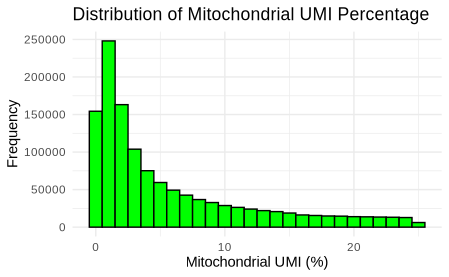
\includegraphics[height=0.2\textheight, width=0.7\textwidth]{000018.png}
  \caption{Distribution of Mitochondrial UMI Percentage: This figure shows the distribution of mitochondrial UMI percentages across all cells. High mitochondrial content can indicate cell stress or damage, and cells with more than 5\% mitochondrial content were filtered out to improve data quality.}
  \label{fig:mito_umi_percent}
\end{figure}

\subsubsection{Quality Control (QC):} To assess the quality of each cell QC metrics were calculated. Cells with high mitochondrial content (more than 5\%) or low library size (fewer than 500 unique molecular identifiers, UMIs) were filtered out. Genes expressed in fewer than 10 cells were also removed to eliminate noise from lowly expressed genes \cite{phipson2022propeller}. This rigorous QC process helps in maintaining the integrity of the data and ensures that subsequent analyses are based on reliable information.

\subsubsection{Normalization and Identification of Highly Variable Genes:} To stabilize the variance across the dataset, raw counts were normalized using a log transformation. The \textbf{scran} package was utilized to identify highly variable genes, which are crucial for distinguishing different cell types. For further analysis, the top 2000 most variable genes were selected. Identifying highly variable genes is essential for focusing on the most informative features of the dataset and disregarding genes that have low or no variability under these conditions \cite{stuart2019comprehensive}.

\begin{figure}[H]
  \centering
  \begin{subfigure}[b]{0.45\textwidth}
    \centering
    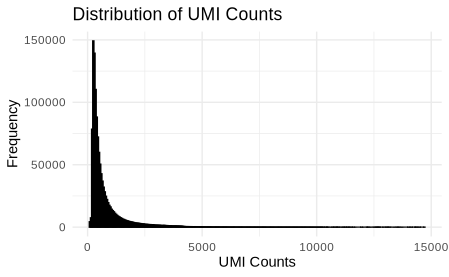
\includegraphics[width=\textwidth]{000016.png}
    \label{fig:mito_umi_before}
  \end{subfigure}
  \hfill
  \begin{subfigure}[b]{0.45\textwidth}
    \centering
    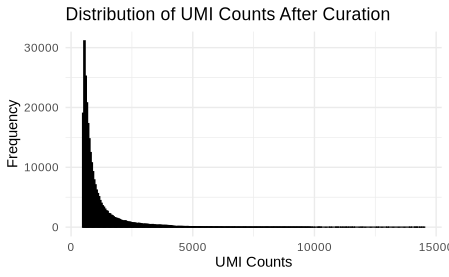
\includegraphics[width=\textwidth]{000010.png}
    \label{fig:umi_counts}
  \end{subfigure}
  \caption{Distribution of UMI Counts After Curation: This figure displays the distribution of UMI counts per cell after quality control and normalization. It shows that most cells have a reasonable number of UMIs, indicating good library complexity and quality after curation}
  \label{fig:umi_distributions}
\end{figure}

\subsection*{Dimensionality Reduction and Clustering}
\subsubsection{Principal Component Analysis (PCA):} PCA was performed on the highly variable genes to reduce the dimensionality of the data. PCA identifies principal components that capture the most significant variations in the dataset. This step is crucial for simplifying the data while retaining its essential patterns \cite{nayak2021hitchhiker}.

\begin{figure}[htbp]
\centering
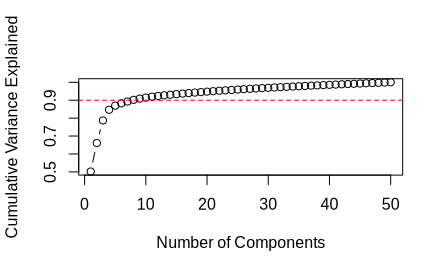
\includegraphics[height=0.2\textheight, width=\textwidth]{000012.png}
\caption{Cumulative Variance Explained by PCA Components: This figure shows the cumulative variance explained by the first 50 principal components. It helps to determine the number of components to retain for further analysis by showing the proportion of variance captured by each component.}
\label{fig_variance}
\end{figure}

\subsubsection{Uniform Manifold Approximation and Projection (UMAP):} UMAP was used to visualize the data in two dimensions. UMAP provides a clearer separation of distinct cell populations compared to PCA, making it easier to identify clusters of similar cells \cite{qiu2017reversed}.

\begin{figure}[htbp]
\centering
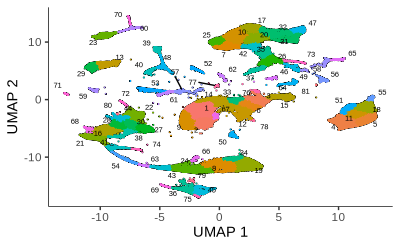
\includegraphics[height=0.3\textheight,width=0.7\textwidth]{umap.png}
\caption{UMAP Visualization of Zebrafish Pigment Cells: This UMAP plot shows the distribution of zebrafish pigment cells in a two-dimensional space, with each point representing a single cell. The colors represent different clusters, indicating distinct cell populations.}
\label{fig_umap_dimensions}
\end{figure}

\subsubsection{Clustering Analysis:} Clustering analysis was conducted to identify distinct cell populations. Clusters were determined based on the principal components from PCA and the UMAP projections. This step involved using algorithms such as Louvain or Leiden for community detection in the data, which help in grouping cells with similar expression profiles \cite{street2018slingshot}.

\begin{figure}[H]
  \centering
  \resizebox{0.4\textheight}{!}{%
    \begin{tabular}{ccc}
      \begin{subfigure}[b]{0.3\textwidth}
        \centering
        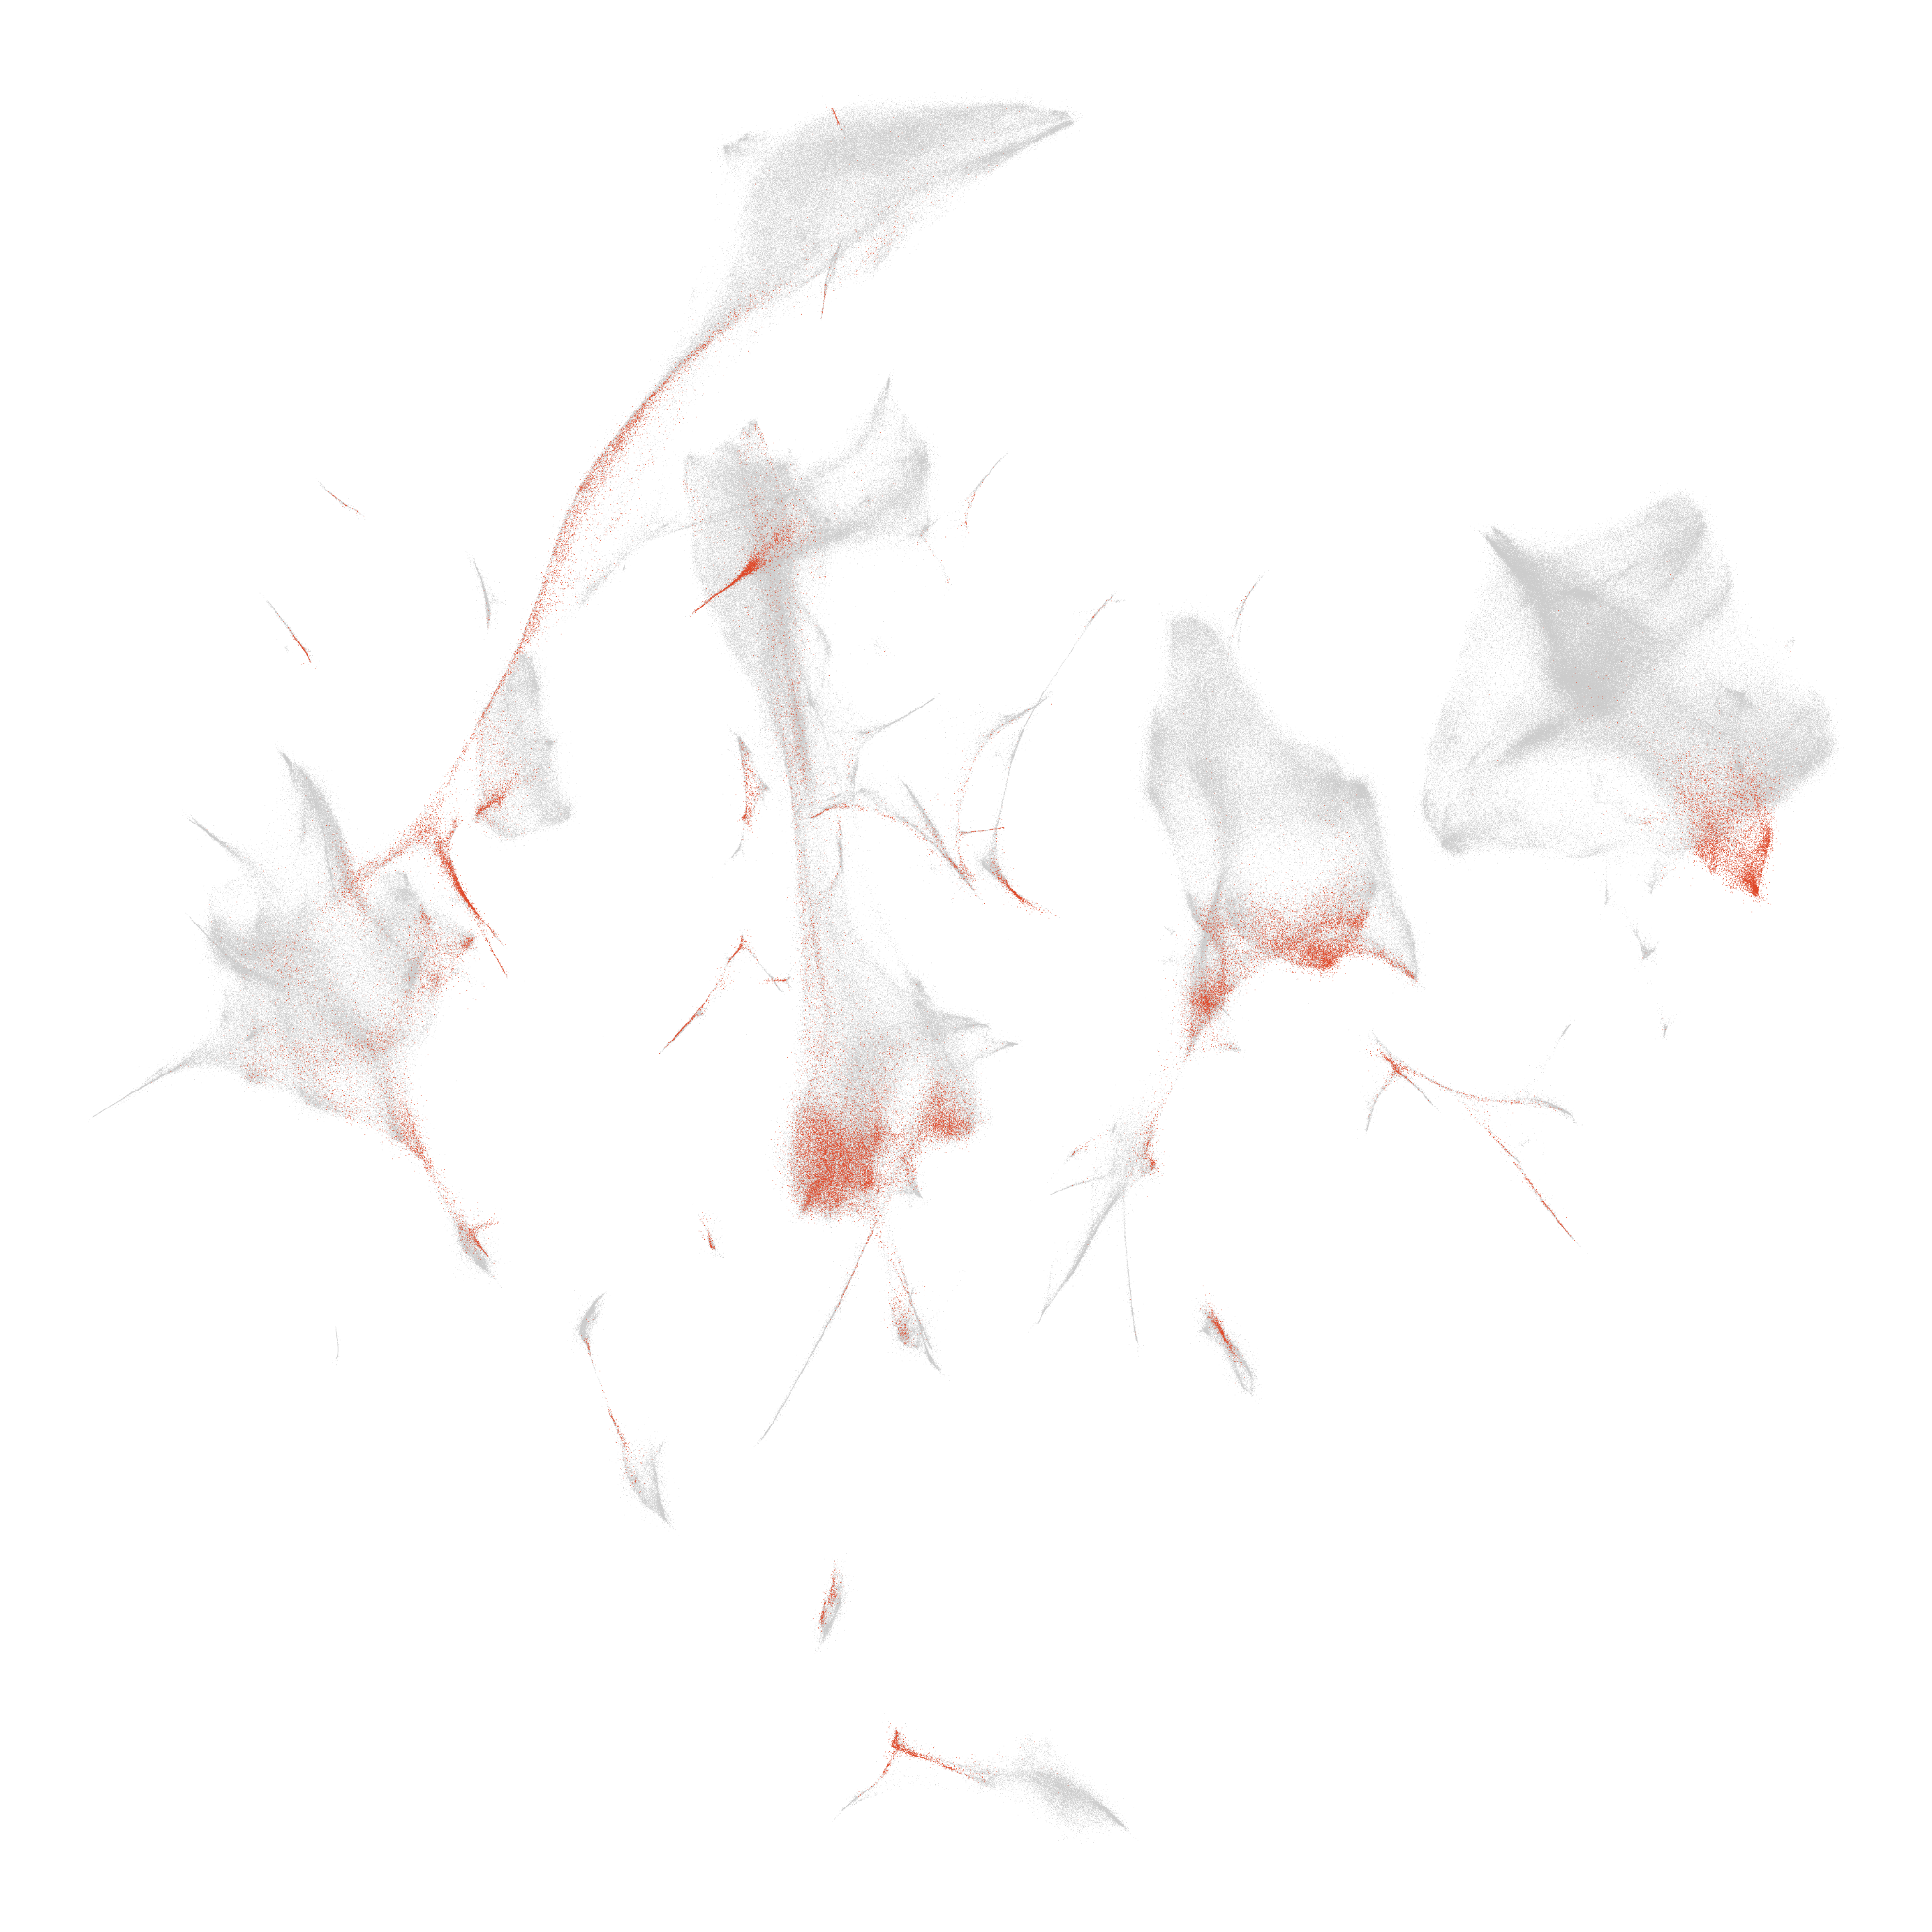
\includegraphics[width=\textwidth]{fig_umap_18h_optimized.png}
        \caption{18h}
        \label{fig:umap_18h}
      \end{subfigure} &
      \begin{subfigure}[b]{0.3\textwidth}
        \centering
        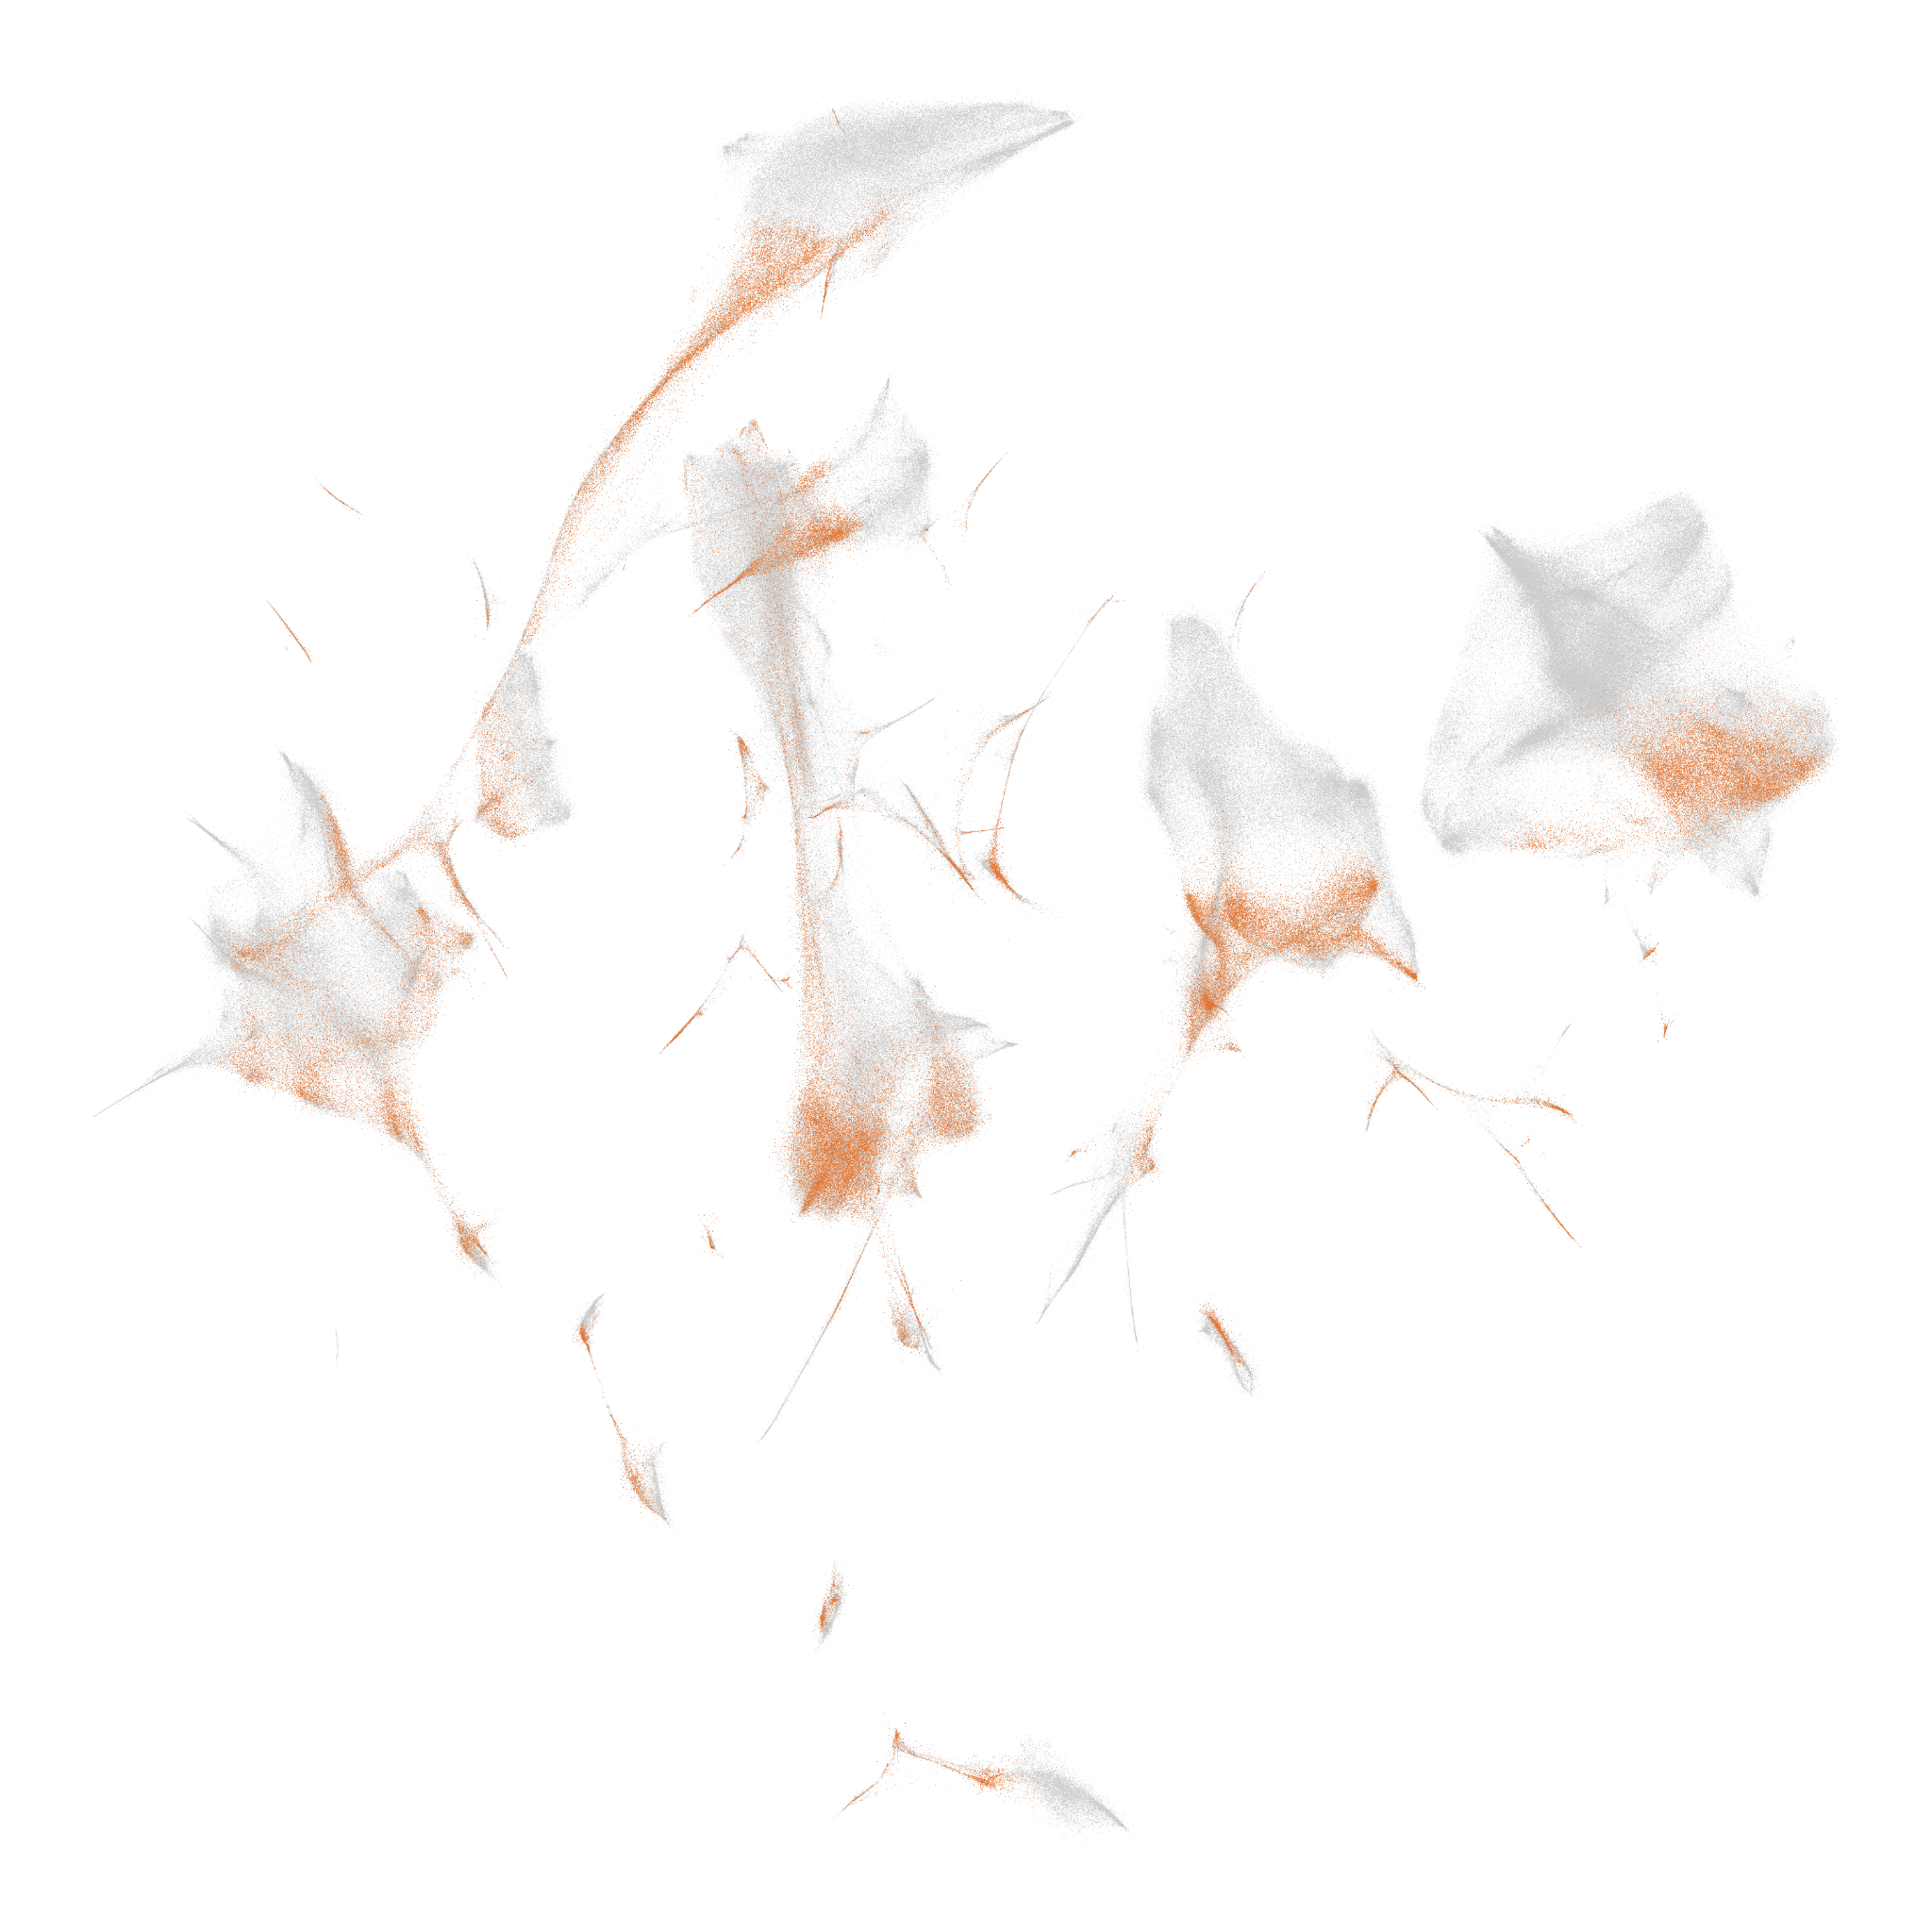
\includegraphics[width=\textwidth]{fig_umap_24h_optimized.png}
        \caption{24h}
        \label{fig:umap_24h}
      \end{subfigure} &
      \begin{subfigure}[b]{0.3\textwidth}
        \centering
        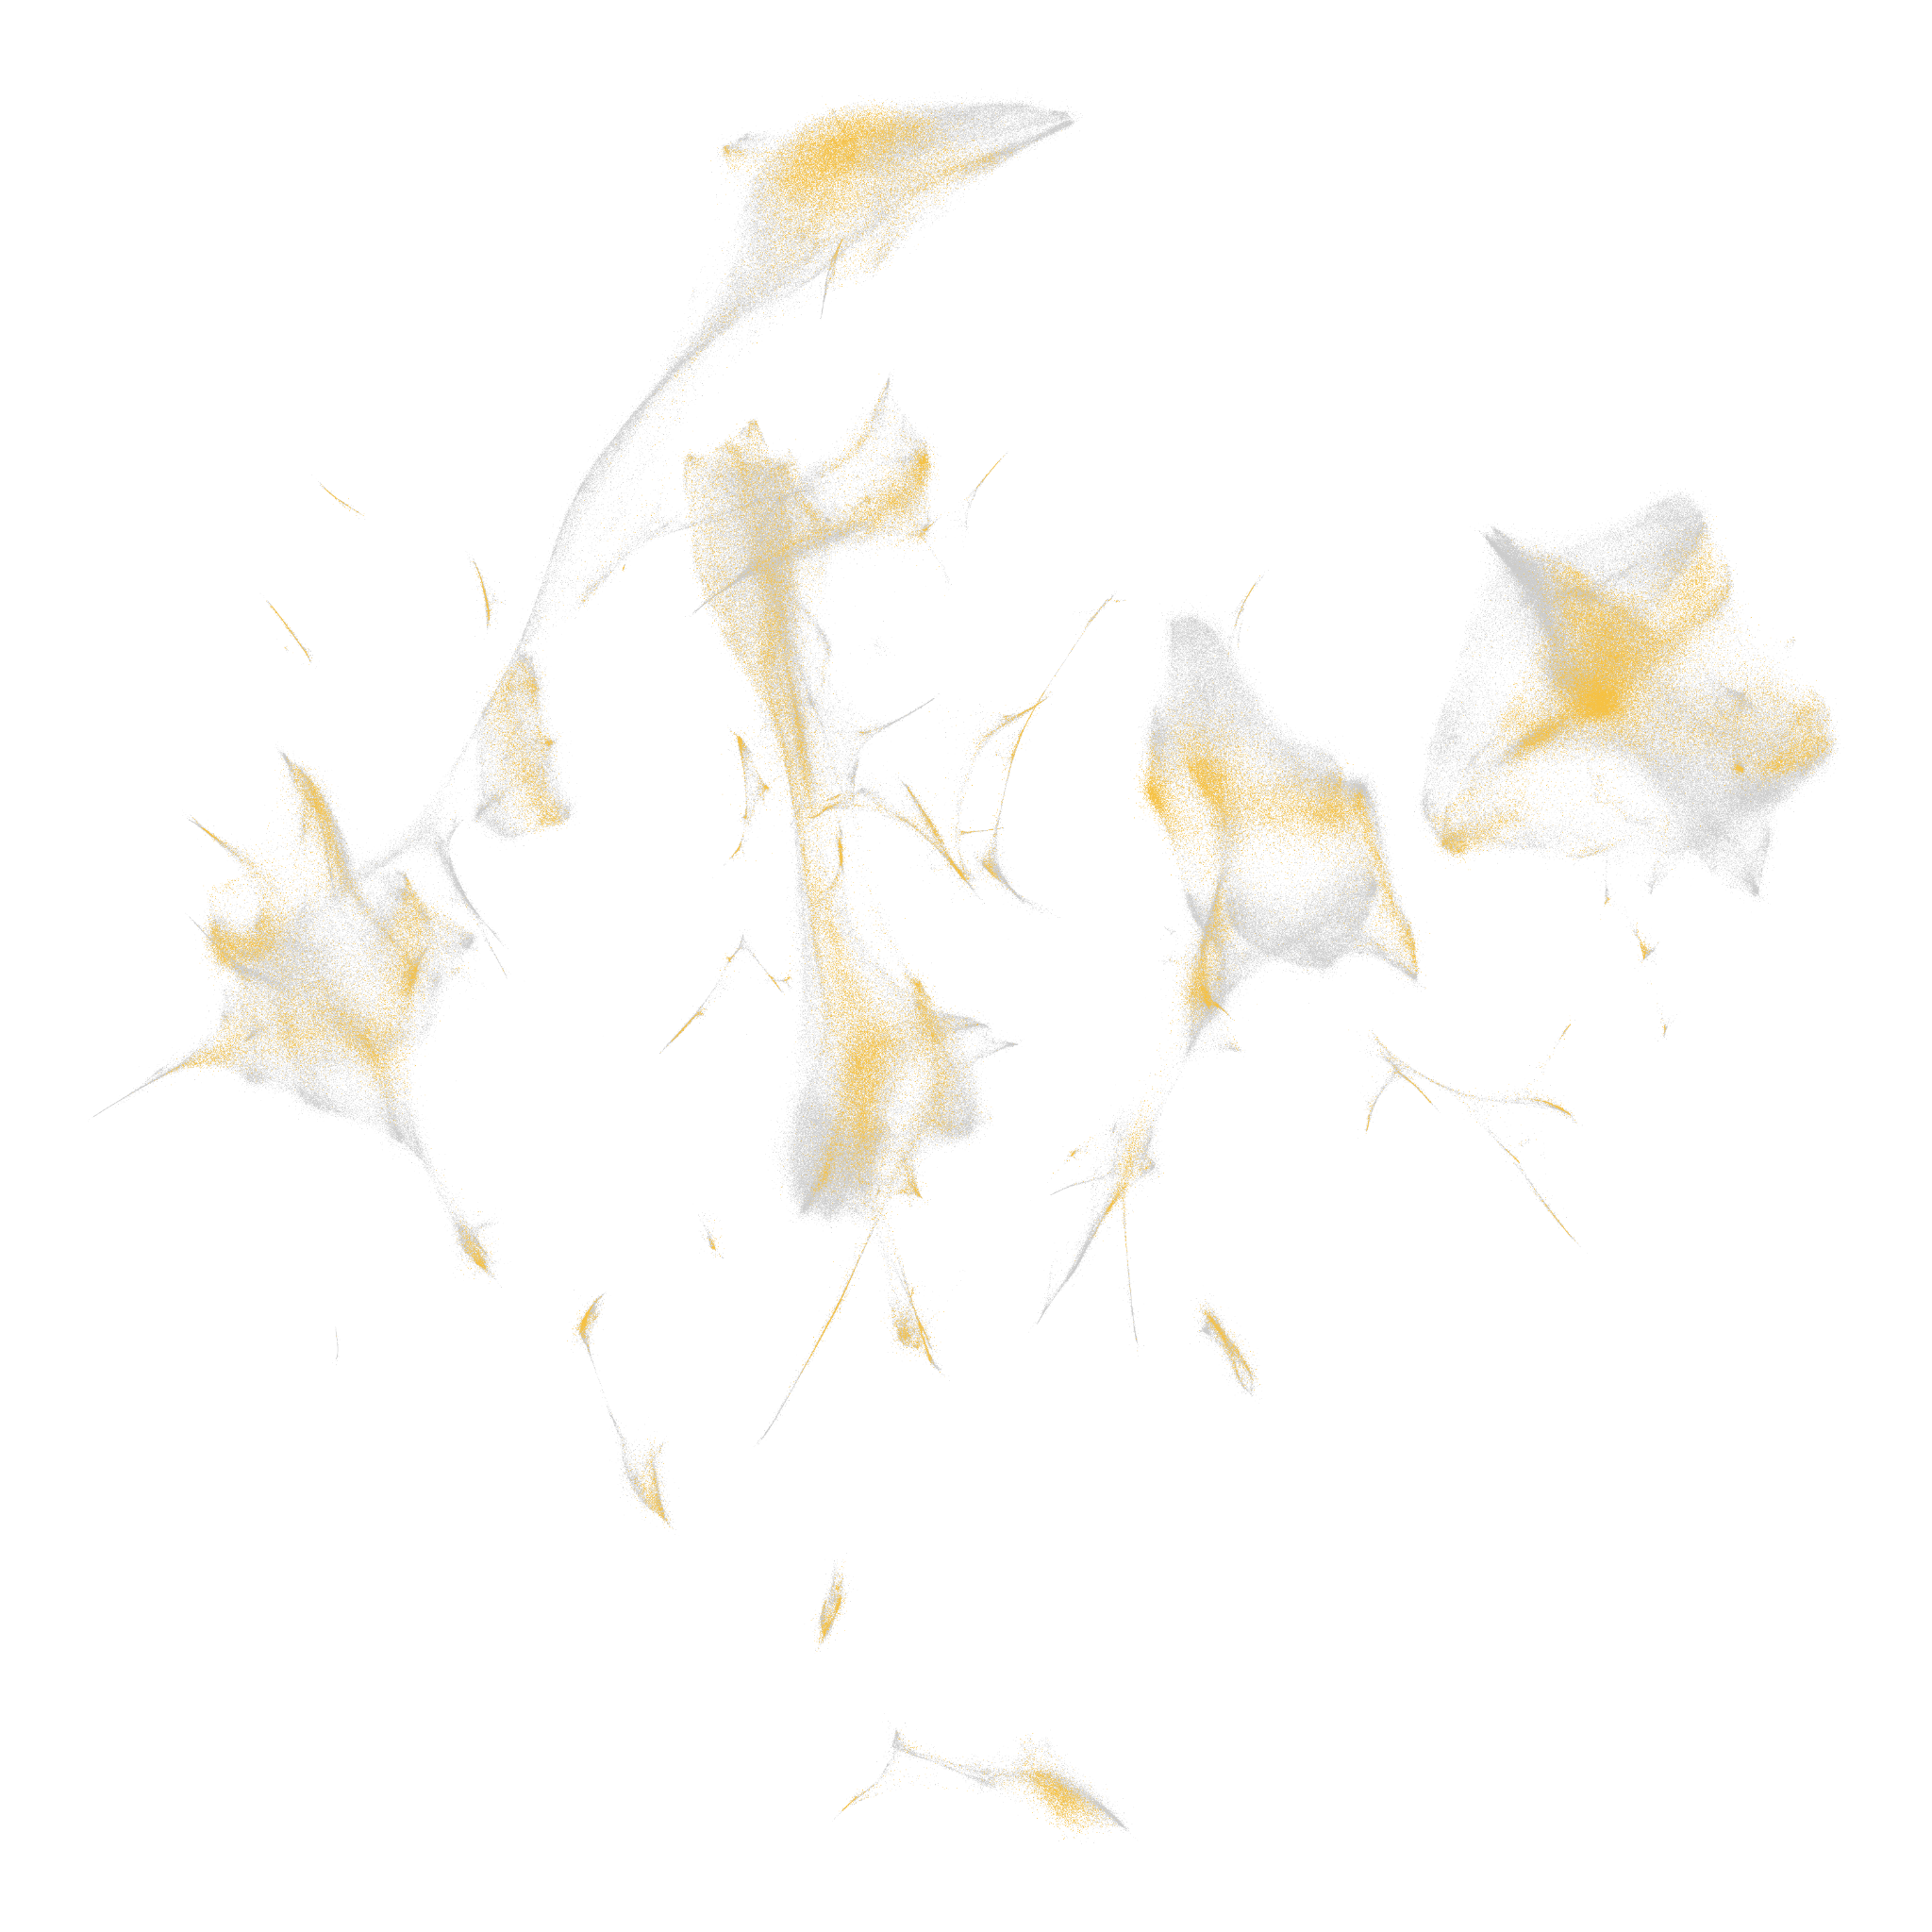
\includegraphics[width=\textwidth]{fig_umap_36h_optimized.png}
        \caption{36h}
        \label{fig:umap_36h}
      \end{subfigure} \\
      \begin{subfigure}[b]{0.3\textwidth}
        \centering
        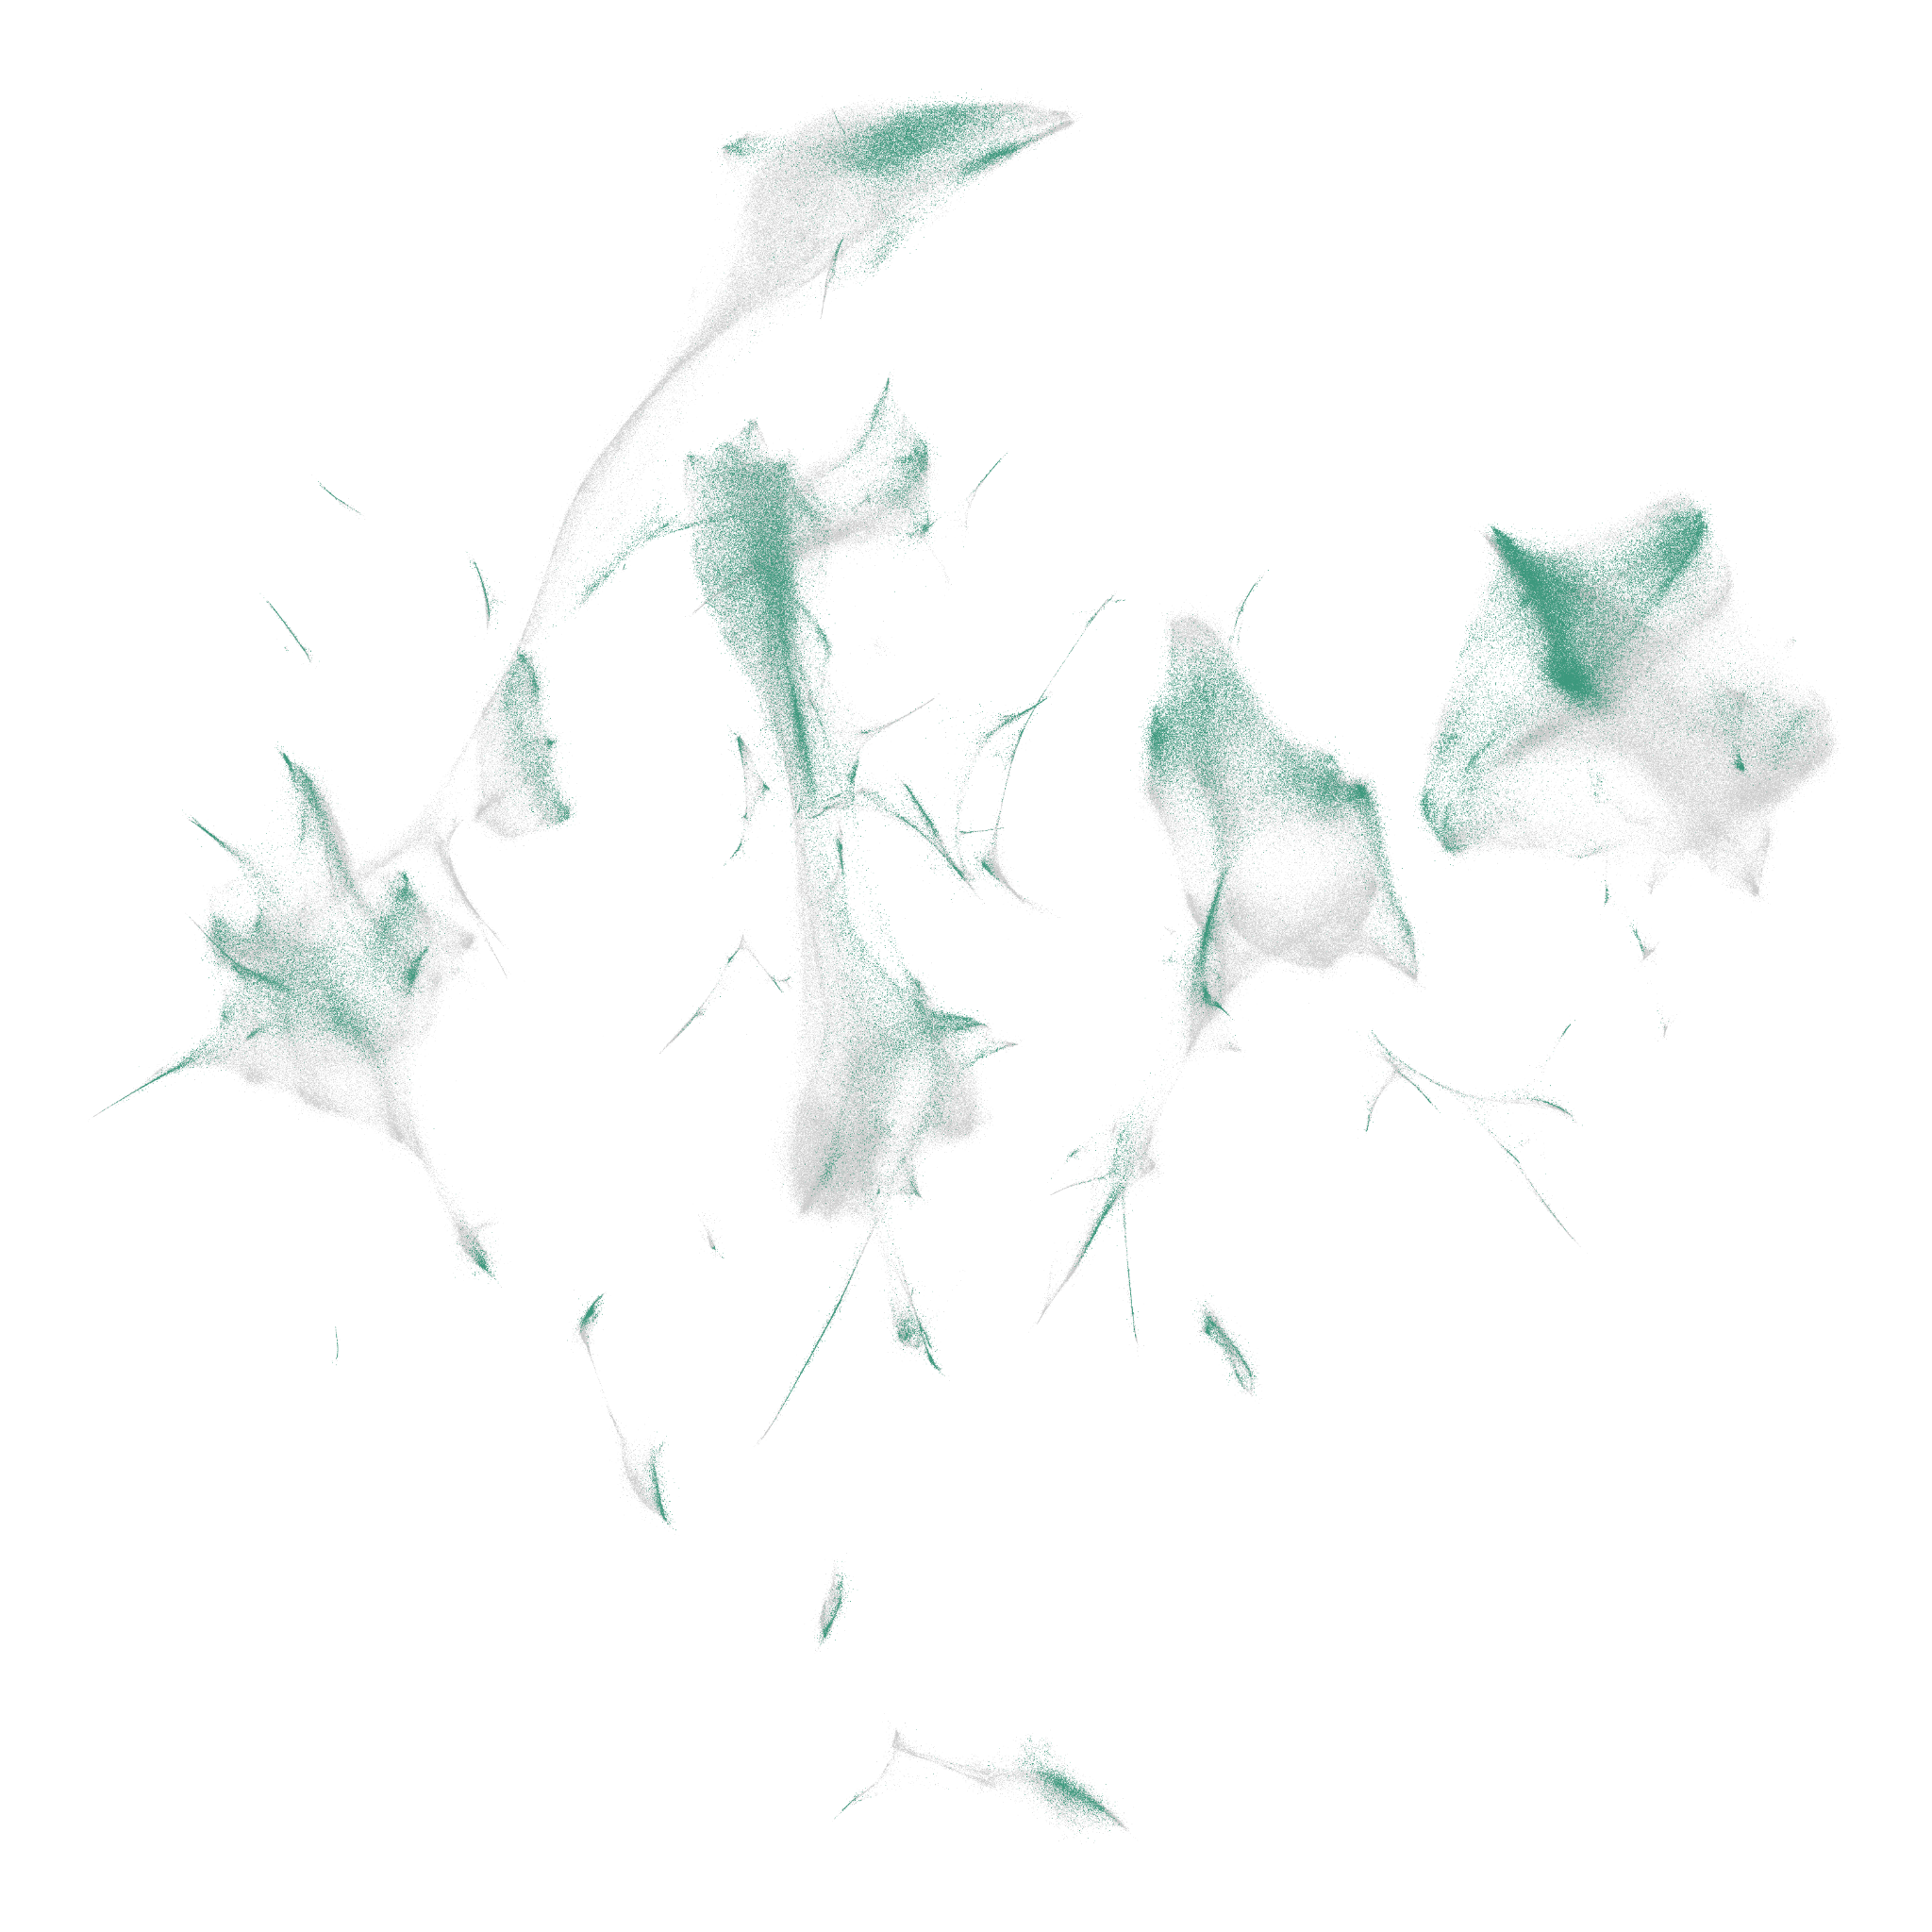
\includegraphics[width=\textwidth]{fig_umap_48h_optimized.png}
        \caption{48h}
        \label{fig:umap_48h}
      \end{subfigure} &
      \begin{subfigure}[b]{0.3\textwidth}
        \centering
        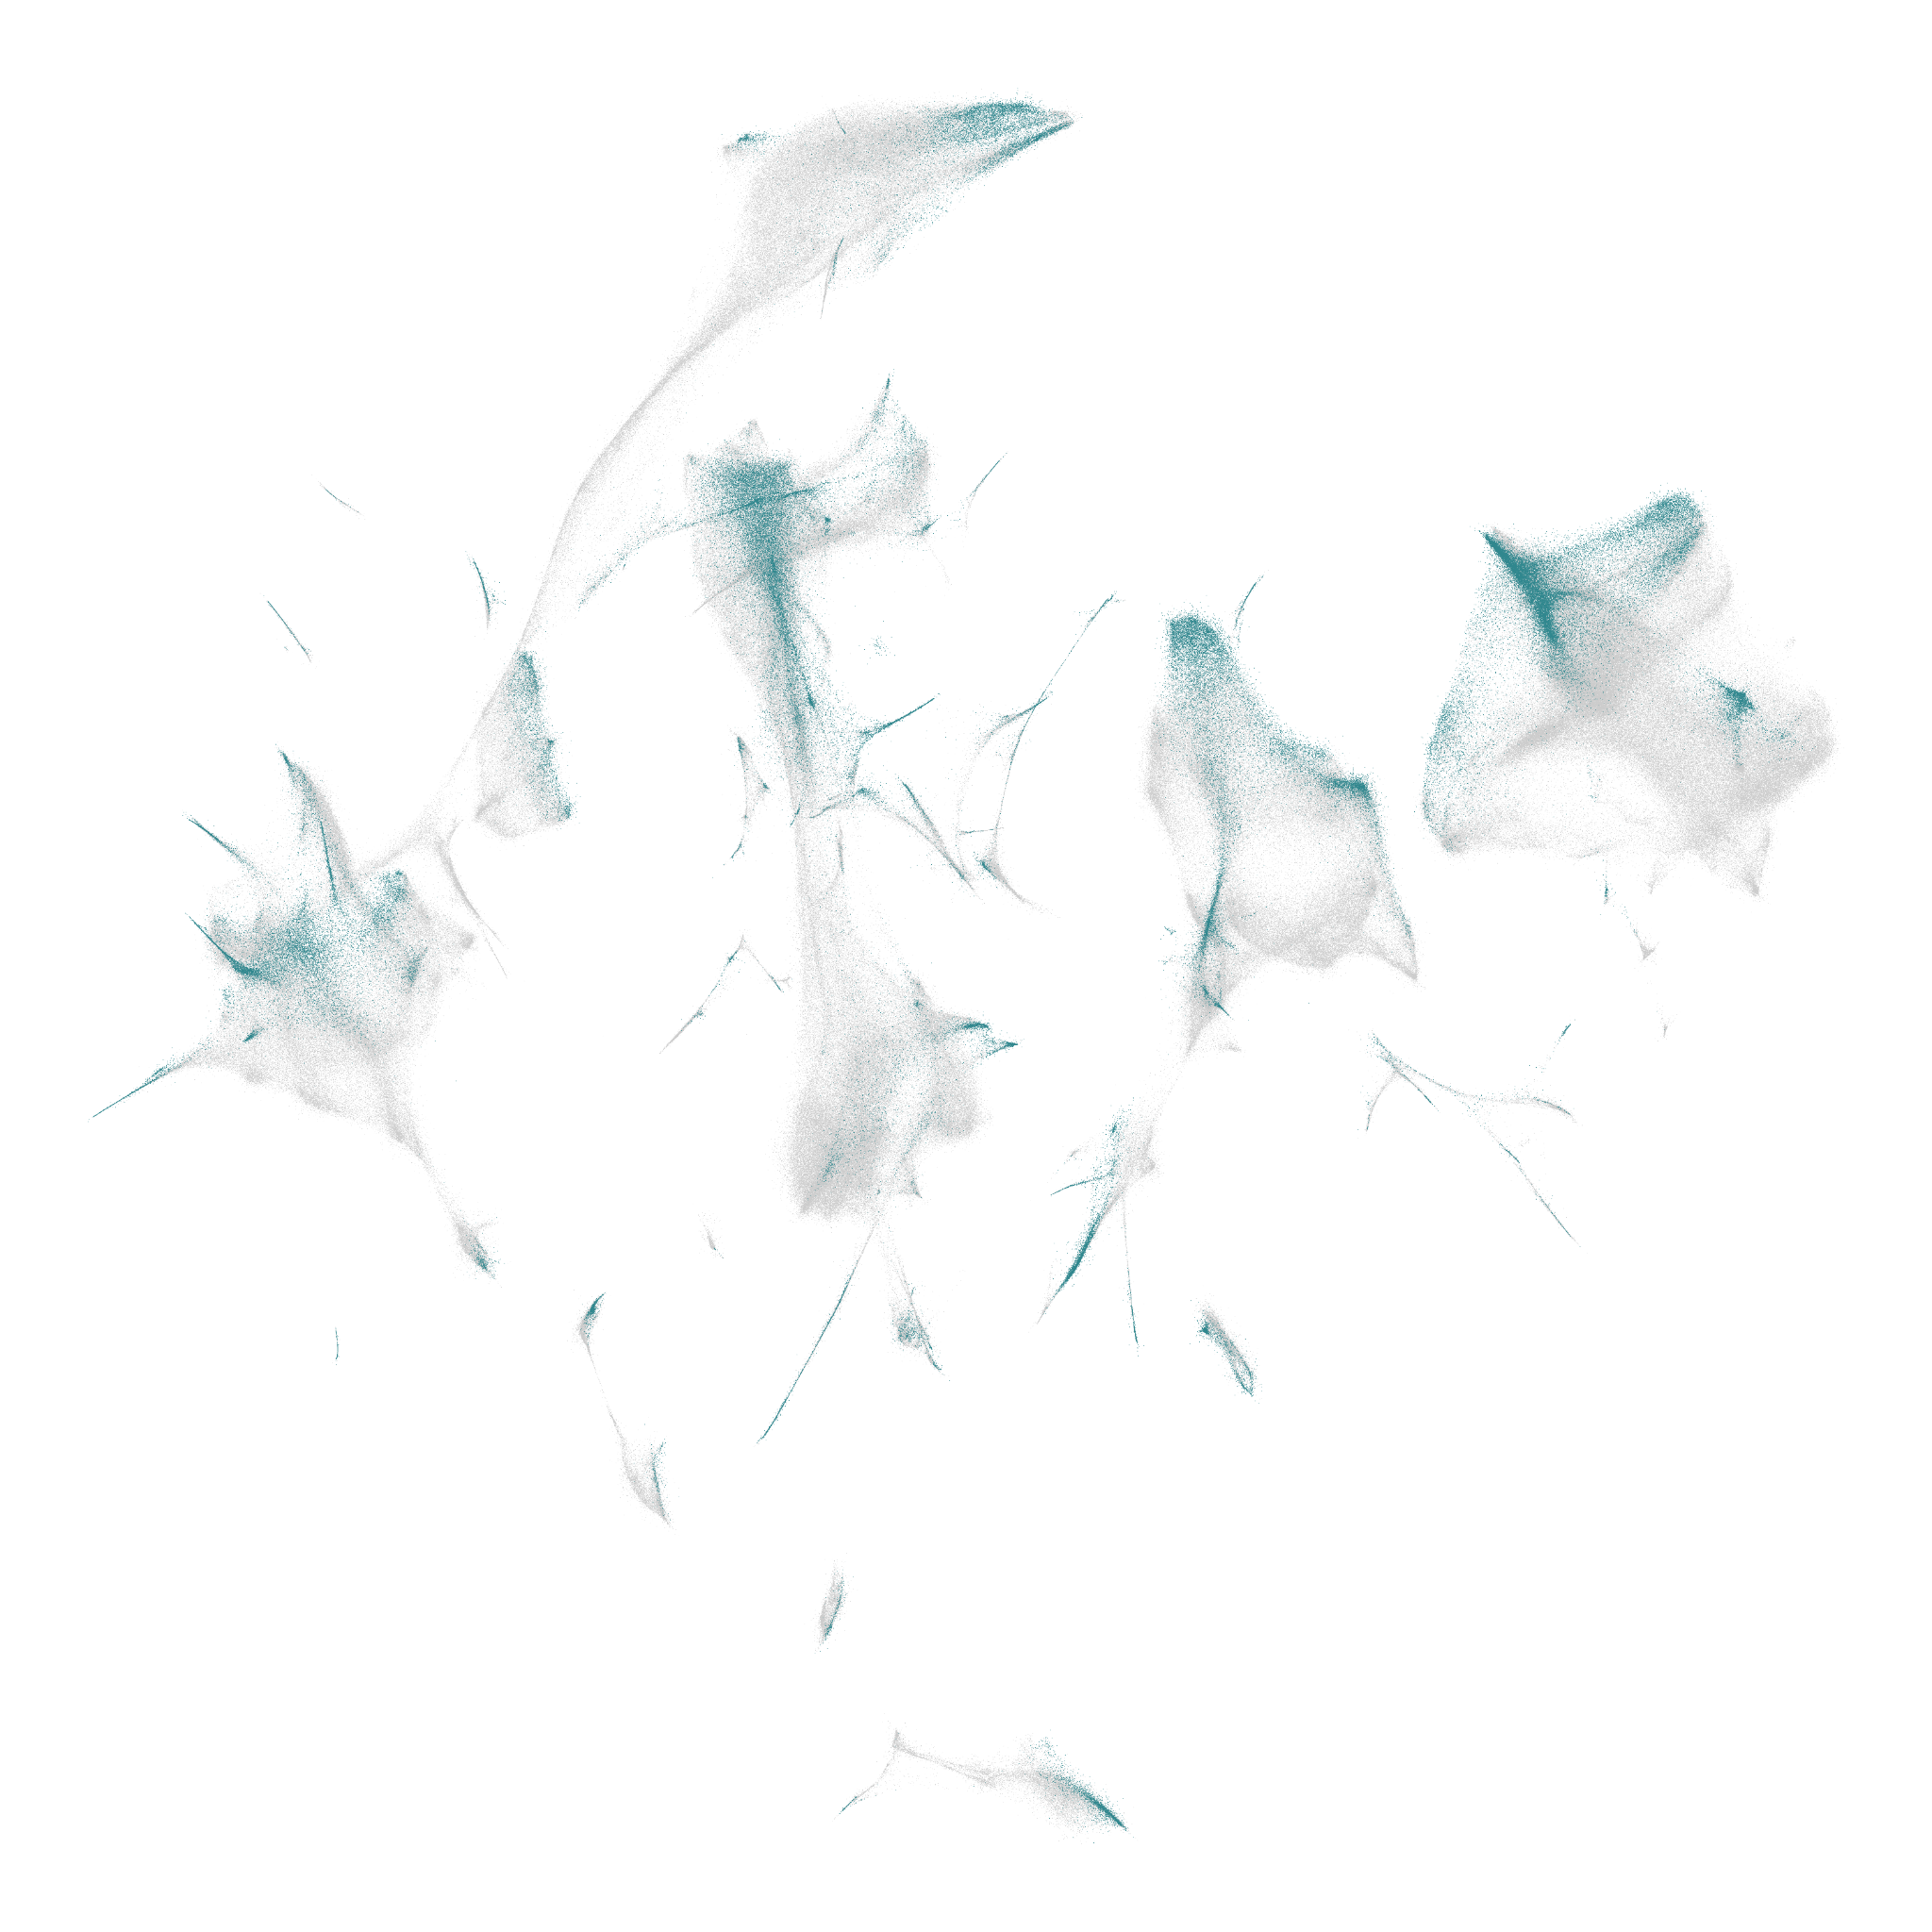
\includegraphics[width=\textwidth]{fig_umap_72h_optimized.png}
        \caption{72h}
        \label{fig:umap_72h}
      \end{subfigure}
    \end{tabular}%
  }
  \caption{UMAP visualizations of zebrafish pigment cells over time (18h-72h), showing the clustering of cells at different developmental stages. Each cluster represents a group of cells with similar gene expression profiles, indicating different cell types or states. These could generate a time-lapse analysis.}
  \label{fig:umap_all}
\end{figure}

\subsection*{Functional Analysis and Gene Expression}
\subsubsection{Marker Genes:} For each cluster to characterize the cell types. The expression of key genes, including \textit{mitfa}, \textit{kit}, and \textit{csf1ra}, was visualized to validate their roles in pigment cell development. Marker genes are critical for defining the identity and function of each cell cluster \cite{howard2021atlas}.

\subsubsection{Pathway and Gene Ontology Enrichment Analysis:} Pathway and Gene Ontology (GO) enrichment analyses were performed to identify significant biological processes and pathways associated with the identified clusters. These analyses help in understanding the functional roles of the genes within each cluster and their involvement in pigment cell differentiation and development \cite{kenny2022tfap2}. Enrichment analysis provides insights into the underlying biological mechanisms driving the observed gene expression patterns.

\section{Results \& Discussion}

The single-cell transcriptome investigation of zebrafish pigment cells aimed to reveal cellular heterogeneity and gene expression patterns. The expectation was to identify highly variable genes that are critical regulators of pigment cell development and to gain insights into the biological mechanisms at work through pathway and GO enrichment studies. However, several challenges were encountered during the analysis:\newline\textbf{Computational Challenges:} The volume of data was significant, and the pre-processing steps required substantial computational resources. The scripts developed to process the scRNA-seq data faced multiple issues, including memory limitations and long execution times.\newline\textbf{Resource Limitations:} The analysis was constrained by the available computational resources. Despite access to a remote computer with better specifications in the final two weeks, the processing times for some scripts were still prohibitively long, ranging from 2 to 24 hours.\newline\textbf{Dataset Selection:} The chosen dataset for the analysis was not ideal for the given computational constraints. Single-cell RNA sequencing analyses generally require extensive computational power and memory, making it challenging to complete within the limited timeframe and resources.

Given these challenges, only a limited number of results were obtained, including a few visualizations of QC metrics, UMI counts, PCA, and UMAP.

Despite the challenges and limitations, the analysis provided some preliminary insights into the cellular heterogeneity and gene expression patterns of zebrafish pigment cells. The quality control steps ensured that only high-quality cells were included in the analysis, and the normalization process allowed for accurate comparison of gene expression levels across cells. The PCA and UMAP visualizations revealed distinct clusters of cells, suggesting the presence of different cell types or states within the pigment cell population.

High-throughput single-cell transcriptomics has revealed previously unknown details on the cellular diversity of tissues in various organisms. According to Kulkarni \textit{et al.} (2019), single-cell RNA sequencing provides an unbiased insight into the cellular makeup of complex tissues, addressing the stochastic nature of gene expression often overlooked in bulk tissue studies \cite{kulkarni2019beyond}.

Trajectory inference is a crucial aspect of single-cell RNA-seq analysis. Qiu \textit{et al.} (2017) presented Monocle 2, an algorithm utilizing reversed graph embedding to express numerous fate decisions in an unsupervised manner, effectively resolving complex single-cell trajectories \cite{qiu2017reversed}. This method has been instrumental in studies of blood formation and other biological processes.

Patterson and Parichy's (2019) examination of zebrafish pigment pattern creation revealed the arrangement and interaction of melanophores, xanthophores, and iridophores for zebrafish stripe formation. Genetic factors such as transcription factors \textit{mitfa}, \textit{tfec}, and receptor tyrosine kinases \textit{kita} and \textit{ltka} are essential for pigment cell differentiation \cite{patterson2019zebrafish}.

\begin{figure}[H]
\centering
\includegraphics[height=0.7\textheight, width=0.7\textwidth]{varianciatotal_boxplot.png}
\caption{Box plot of total variance in gene expression. This box plot summarizes the overall variance in gene expression levels across different cell types, providing insights into the heterogeneity within the pigment cell population.}
\label{results 1}
\end{figure}

Saunders \textit{et al.} (2023) conducted a comprehensive single-cell transcriptome investigation of developing zebrafish embryos, resulting in a high-resolution map of cell type compositions and developmental trajectories. Their dataset, which includes 1812 embryos and 3.2 million cells, allows for the estimation of cell type abundance variation and discovery of perturbation-dependent variances in cell type composition. This robust dataset provides a framework for understanding the genetic connections and developmental processes of zebrafish pigment cells \cite{saunders2023embryo}.

\begin{figure}[H]
  \centering
  \includegraphics[height=0.2\textheight, width=0.5\textwidth]{variancia_tempos.png}
  \caption{Variance of gene expression over different time points. This plot shows the variance in gene expression for various genes across different developmental stages, highlighting the dynamic nature of gene regulation during pigment cell development.}
  \label{results 2}
\end{figure}

Additionally, Saunders \textit{et al.} (2019) elucidated the influence of thyroid hormone on pigment cell line maturation, showing that hormone signaling pathways significantly impact pigment cell formation and differentiation, consistent with our pathway enrichment findings \cite{saunders2019thyroid}.

Phipson \textit{et al.} (2022) used propeller to evaluate variations in cell type proportions in single-cell data, demonstrating the resilience of statistical approaches for evaluating scRNA-seq datasets. This method validated the quality control and clustering results from our study \cite{phipson2022propeller}.

The following figures illustrate the key findings from replicating Saunders \textit{et al.} (2023) processed code, datasets and tables and the last image was generated by me after isolating a small subsample of transcription factors over time, and it was very memory intensive as well.

\begin{figure}[H]
  \centering
  \includegraphics[height=0.25\textheight, width=0.6\textwidth]{expression_of_genes_in_pigment_cells_over_time.png}
  \caption{Expression of genes in pigment cells over time. This graph shows the mean expression levels of various genes involved in pigment cell development across different time points, highlighting dynamic changes in gene expression.}
  \label{results 3}
\end{figure}

\section{Conclusion}

This study utilized high-quality single-cell RNA-seq data to understand the zebrafish pigment cell transcriptome better. Initial analysis steps, including data processing and normalization, were completed, but the full analysis faced limitations due to computational constraints. Nonetheless, the study provided valuable preliminary insights into the genetic regulation of pigmentation and highlighted the importance of adequate computational resources for single-cell RNA-seq analysis. Future work could involve experimental validation of these findings and the integration of additional datasets to create a more comprehensive perspective.

\section{Future Work}
To address the issues encountered and complete the analysis, the following steps are recommended:\newline\textbf{Enhanced Computational Resources}: Utilize a high-performance computing cluster with sufficient memory and processing power to handle large single-cell RNA-seq datasets.\newline\textbf{Optimized Scripts}: Refine and optimize the scripts for better performance and efficiency.\newline\textbf{Extended Timeframe}: Allocate more time for the analysis to allow for the completion of all pre-processing and downstream analysis steps.\newline\textbf{Experimental Validation}: Validate the findings experimentally to ensure the accuracy and relevance of the results.\newline\textbf{Integration of Additional Datasets}: Incorporate additional datasets to create a more comprehensive understanding of zebrafish pigment cell development.

In conclusion, while the analysis faced significant challenges and was not fully completed, the experience provided valuable insights into the complexities and requirements of single-cell RNA sequencing studies. Future work with enhanced resources and an optimized approach will be essential to achieving the study's objectives.

\section*{Acknowledgements}
I am grateful to David Henriques of CSIC IIM in Vigo and Professor Miguel Rocha of the University of Minho in Braga for the chance and collaboration on this research project. I also want to thank my family, friends, and colleagues for their useful advices and support over the first year of my Masters degree in Bioinformatics, as this is my final course during this academic year.

\newpage
\bibliographystyle{splncs04}
\bibliography{references}

\end{document}